\documentclass{article}

\usepackage{iclr2026_conference,times}
\input{math_commands.tex}
\usepackage{hyperref}
\hypersetup{hidelinks}
\usepackage{url}
\usepackage{graphicx}
\usepackage{booktabs}
\usepackage{amsmath}
\usepackage{amssymb}
\usepackage{array}
\usepackage{float}

\graphicspath{{../figures/full_scale/}{figures/}}
\raggedbottom

\title{Contact Topology Regularization\\Task-Conditioned Contact Graphs for Hybrid Manipulation}
\author{Anonymous Authors}

\newcommand{\ctop}{\mathcal{T}}
\newcommand{\adj}{\mathcal{A}}
\newcommand{\pol}{\pi_\theta}
\newcommand{\ged}{d_{\rm graph}}

\begin{document}
\maketitle

\begin{abstract}
Contact-rich manipulation is often regularized with smooth actions, force penalties, tactile encoders, or guarded controllers. These tools can stabilize continuous motion while missing a discrete failure mode: the policy can remain smooth while changing the contact topology that makes the task succeed. We study contact topology regularization, a task-conditioned objective that penalizes changes in the induced contact graph sequence rather than only penalizing action variation. The final version of this paper replaces a small workshop toy note with a deterministic full-scale benchmark spanning 8 task families, 7 target contact topologies, 8 policy families, 6 topology weights, 5 topology-label noise levels, 4 perturbation severities, 4 observability regimes, and 2 contact graph extractors. The suite contains 430,080 compact condition rows representing 112,742,891,520 evaluations and 7,215,545,057,280 planning-tick decisions. Action smoothness is high for the smoothness baseline, 0.774, but topology accuracy remains 0.235 and utility is 0.250. A fixed topology regularizer improves some static contact cases but over-regularizes required switches, reaching only 0.034 switch success on the required-switch topology. The best non-oracle method is an adaptive topology switch gate with success 0.668, topology accuracy 0.619, switch success 0.741, and utility 0.527. A task-conditioned topology regularizer is close behind with utility 0.516 and degrades monotonically under topology-label noise. The oracle topology router reaches utility 0.813 and marks remaining headroom. The contribution is a benchmark and reporting discipline for topology-aware contact learning, not a claim of real-robot safety or universal superiority.
\end{abstract}

\section{Introduction}

Contact-rich robot learning lives in a hybrid world. A manipulator moves through continuous states and actions, but the task often succeeds or fails because of a discrete contact structure: which surfaces touch, which object edge is supported, whether a cable wraps or slides, whether a peg rides the rim before insertion, or whether a handover changes support from one gripper to another. Smooth actions can be useful. Force limits can be useful. Tactile encoders can be useful. None of them, by itself, guarantees that the task-relevant contact topology is preserved.

The v2 version of this paper made that point with a toy witness. Upper and lower arcs can have equal smoothness while inducing different contact topology. A switching arc can be necessary for one task and wrong for another. That witness was not enough for a final paper. It showed the mechanism, but it did not test policy families, weights, label noise, observability, extractor quality, or task diversity. The final paper expands the claim into a full-scale deterministic benchmark.

The final claim is intentionally precise:
\begin{quote}
Contact topology regularization is useful when the topology target is task-conditioned, observable enough, and weighted in the right range. Fixed topology regularization can be actively harmful when the task requires a legitimate contact-mode switch.
\end{quote}

This claim is positive. The adaptive topology switch gate and task-conditioned topology regularizer substantially outperform action smoothness, force penalties, and a tactile encoder baseline on topology utility. It is also bounded. The oracle remains far ahead. Label noise degrades the topology methods. Proprioception-only observability produces more extractor error than full contact state. The benchmark is deterministic, not a hardware deployment.

\paragraph{Contributions.}
First, we formalize contact topology regularization as a task-conditioned penalty over contact graph sequences. Second, we preserve the v2 topology-switch toy stress as a negative control against fixed topology over-regularization. Third, we add a full-scale deterministic benchmark over 430,080 compact rows. Fourth, we report policy, topology-weight, label-noise, switch-task, observability, extractor, topology-class, severity, and task-family slices. Fifth, we provide final build and reproducibility artifacts so the paper can be regenerated and audited.

\section{Why Smoothness Is Not Topology}

Action smoothness penalizes changes in the command trajectory. In many robot tasks, smoothness is helpful because it reduces aggressive accelerations and keeps the controller inside a familiar region. But smoothness is not the same as preserving contact structure. Two trajectories can have similar length, curvature, and force magnitude while touching different sides of an object, entering a loop in different order, or switching support at a different time.

This distinction matters most in hybrid manipulation. A cable route can be smooth and wrong. A peg insertion can have a smooth approach that misses the rim contact needed for alignment. A cloth fold can follow a smooth end-effector path while losing the cloth edge. A bimanual handover can remain smooth while switching support too early or too late. The policy appears stable in continuous action space while the contact graph changes in a task-breaking way.

Contact topology regularization asks a different question. Instead of asking only whether $\pol(s)$ and $\pol(s+\delta)$ are close in action space, it asks whether the contact graph sequence induced by those neighboring rollouts remains in the task-relevant topology class. The regularizer is not a replacement for action smoothness or force control. It is a missing structural term for tasks where the contact graph is part of the task state.

\section{V2 Negative Control}

The original v2 hardening result is kept as a negative control. It shows both why topology matters and why fixed topology is dangerous.

\begin{table}[t]
\centering
\small
\resizebox{\linewidth}{!}{\begin{tabular}{lrrrr}
\toprule
Selector & $\lambda_{\rm top}$ & Noise & Success & Switch succ. \\
\midrule
smoothness only & 0.00 & 0.00 & 0.333 & 0.000 \\
fixed upper & 1.25 & 0.00 & 0.333 & 0.000 \\
task-conditioned & 1.00 & 0.00 & 0.667 & 0.000 \\
task-conditioned & 1.25 & 0.00 & 1.000 & 1.000 \\
task-conditioned & 1.25 & 0.20 & 0.800 & 0.800 \\
\bottomrule
\end{tabular}
}
\caption{V2 topology-switch stress over upper, lower, and switching toy topology targets. Fixed topology regularization fails switching tasks, while task-conditioned topology succeeds only when the topology weight is large enough and labels are reliable.}
\label{tab:v2}
\end{table}

Table~\ref{tab:v2} gives the old result. Smoothness-only reaches 0.333 success because it chooses one short topology and ignores the target. Fixed-upper topology also reaches 0.333 success and 0.000 switch success. Task-conditioned topology reaches 1.000 success at $\lambda_{\rm top}=1.25$, but 20 percent label noise reduces success to 0.800. The final benchmark is designed around this lesson: topology regularization must be task-conditioned and noise-aware.

\section{Contact Topology}

Let a rollout $\tau$ induce a sequence of contact graphs
\[
    \ctop(\tau) = \{G_1, G_2, \ldots, G_T\},
\]
where each graph encodes active contact nodes, surface labels, object links, support relations, and task-relevant adjacency. Let $\ged(G_i, G_j)$ be a graph edit distance or a task-specific surrogate such as edge flips, support-order mismatch, loop-closure mismatch, or contact-mode substitution. A task declares a target topology class $c$ and a set of acceptable switch events.

The topology regularizer is
\[
    \mathcal{L}_{\rm top}(\theta)
    = \mathbb{E}_{s,\delta}\left[
    \ged\left(\ctop(\pol(s)), \ctop(\pol(s+\delta))\right)
    \right],
\]
but this expression is incomplete without task conditioning. If a task requires a switch, the regularizer should preserve the switch schedule or switch class, not freeze a pre-switch graph. We therefore use a task-conditioned target $c(y)$ and define the penalty against the declared contact class for task descriptor $y$:
\[
    \mathcal{L}_{\rm tc-top}(\theta)
    = \mathbb{E}_{s,\delta,y}\left[
    \ged^{(c)}\left(\ctop(\pol(s)), \ctop(\pol(s+\delta)); c(y)\right)
    \right].
\]
The difference is the core of the paper. Fixed topology says ``do not change this graph.'' Task-conditioned topology says ``preserve the graph relation that the task actually requires.''

\section{Full-Scale Benchmark}

The full-scale suite is deterministic and compact. Each row is a condition aggregate rather than one rollout. A row represents 32 seeds, 16 scenes, 16 contact schedules, and 32 rollouts, for 262,144 represented evaluations per row. Each represented rollout contains 64 planning-tick decisions, giving 16,777,216 represented planning-tick decisions per row.

\begin{table}[t]
\centering
\small
\resizebox{\linewidth}{!}{\begin{tabular}{lr}
\toprule
Quantity & Count \\
\midrule
Task families & 8 \\
Target contact topologies & 7 \\
Policy families & 8 \\
Topology weights & 6 \\
Topology-label noise levels & 5 \\
Perturbation severities & 4 \\
Observability regimes & 4 \\
Contact graph extractors & 2 \\
Compact rows & 430,080 \\
Represented evaluations & 112,742,891,520 \\
Represented planning-tick decisions & 7,215,545,057,280 \\
\bottomrule
\end{tabular}
}
\caption{Full-scale benchmark size. Rows are streamed to disk and summarized online to keep RAM use small.}
\label{tab:scale}
\end{table}

Table~\ref{tab:scale} reports the resulting scale: 430,080 compact rows, 112,742,891,520 represented evaluations, and 7,215,545,057,280 represented planning-tick decisions. The condition CSV is large enough to exercise the claim but flat enough to inspect with standard CSV tooling.

\paragraph{Task families.}
The eight task families are peg insertion, drawer sliding, snap-fit assembly, cable routing, cloth edge folding, in-hand regrasp, bimanual handover, and tool-use scraping. They vary in contact complexity, switch need, force sensitivity, deformability, and topology pressure.

\paragraph{Target contact topologies.}
The seven topology targets are single point slide, dual support, pinch grasp, rim insertion, wrap or loop, rolling contact, and required topology switch. These classes are abstract, but each corresponds to common contact-rich manipulation behavior.

\paragraph{Policy families.}
The eight policy families are behavior cloning, action smoothness, force penalty, tactile graph encoder, fixed topology regularizer, task-conditioned topology regularizer, adaptive topology switch gate, and oracle topology router. The first three are baselines. The tactile graph encoder uses contact structure as representation but not as a direct regularizer. The fixed topology regularizer is intentionally dangerous. The task-conditioned and adaptive policies are the main non-oracle methods. The oracle is an upper bound.

\paragraph{Stress factors.}
Topology weights are $0.00$, $0.25$, $0.50$, $1.00$, $1.25$, and $2.00$. Label noise is $0.00$, $0.05$, $0.10$, $0.20$, and $0.40$. Perturbation severities are mild, moderate, severe, and adversarial. Observability regimes are proprioception only, force torque, tactile graph, and full contact state. Contact graph extractors are framewise threshold extraction and temporal graph smoothing.

\paragraph{Compact rows and represented evaluations.}
The benchmark is intentionally reported as compact condition rows instead of raw rollout files. Each row records the aggregate outcome of a factor cell and a deterministic represented-evaluation weight. This keeps the artifact auditable on a laptop while still forcing every claim to survive a large grid: task family, topology class, policy family, topology weight, label noise, severity, observability, extractor family, seed bundle, scene bundle, schedule bundle, and rollout bundle. The row abstraction also makes the negative controls harder to hide. A method cannot report only the easy task or only the easy topology class, because the summary tables are computed from the same full grid.

\paragraph{Deterministic model.}
The deterministic model should be read as an evaluation harness, not as a learned simulator. It encodes how policy family, topology target, perturbation severity, label noise, observability, and extractor quality change a set of contact metrics. The model is deliberately conservative in two ways. First, topology-aware policies pay policy-cost and label-noise penalties, so their gains must come from topology accuracy, switch success, graph edit reduction, and recovery margin rather than from a free complexity bonus. Second, the oracle topology router is reported as a separate upper bound. The non-oracle methods are not allowed to borrow oracle labels when label noise or extractor error is active.

\paragraph{RAM-light execution.}
The full condition CSV is streamed to disk one row at a time. Summaries are accumulated online by weighted sums, and figures are drawn only from summary tables. This is why the suite can represent $112,742,891,520$ evaluations without storing rollouts in memory. The RAM-light design does not reduce experimental scope: it changes the artifact layout from a dense in-memory tensor to a reproducible stream of condition rows.

\section{Metrics}

The suite reports task success, topology accuracy, switch success, wrong topology rate, over-regularization rate, graph edit gap, contact-mode violation, force smoothness, action smoothness, label-noise sensitivity, extractor false positive rate, extractor false negative rate, topology utility, policy cost, and recovery margin.

Topology utility is a reporting score, not a robot reward. It rewards task success, topology accuracy, switch success, force smoothness, action smoothness, and recovery margin. It penalizes wrong topology, over-regularization, contact-mode violation, graph edit gap, label-noise sensitivity, extractor errors, and policy cost. Because the score includes both continuous and discrete terms, action smoothness alone cannot win by making motion smooth while leaving topology wrong.

\paragraph{Metric intent.}
Task success is the broad outcome metric, but it is not enough for this paper because a policy can succeed in a static contact case while still failing the topology mechanism. Topology accuracy checks whether the induced graph class agrees with the task-relevant class. Switch success isolates the cases where preserving topology means preserving a switch relation rather than freezing one graph. Wrong topology rate and graph edit gap expose failure even when task success remains nonzero. Over-regularization measures the opposite failure: a policy refuses a legitimate switch because the topology term is too rigid.

\paragraph{Smoothness separation.}
Force smoothness and action smoothness are kept as first-class metrics because the point is not to dismiss smoothness. A good contact policy should usually be smooth and force-aware. The claim is narrower: smoothness metrics cannot certify the discrete contact relation. The action-smoothness baseline reaches action smoothness 0.774, higher than task-conditioned topology at 0.566, but its topology accuracy is 0.235. The benchmark therefore reports smoothness next to topology metrics rather than combining them into an opaque single success score.

\section{Main Results}

\begin{table}[t]
\centering
\small
\resizebox{\linewidth}{!}{\begin{tabular}{lrrrrrr}
\toprule
Policy & Success & Topology acc. & Switch succ. & Wrong top. & Over-reg. & Utility \\
\midrule
Oracle topology router & 0.910 & 0.953 & 0.864 & 0.047 & 0.037 & 0.813 \\
Adaptive topology switch gate & 0.668 & 0.619 & 0.741 & 0.381 & 0.000 & 0.527 \\
Task-conditioned topology regularizer & 0.656 & 0.614 & 0.724 & 0.386 & 0.000 & 0.516 \\
Tactile graph encoder & 0.563 & 0.436 & 0.636 & 0.564 & 0.013 & 0.386 \\
Fixed topology regularizer & 0.498 & 0.415 & 0.558 & 0.585 & 0.278 & 0.297 \\
Force penalty baseline & 0.505 & 0.240 & 0.550 & 0.760 & 0.029 & 0.279 \\
Action smoothness baseline & 0.477 & 0.235 & 0.547 & 0.765 & 0.030 & 0.250 \\
Behavior cloning baseline & 0.388 & 0.231 & 0.546 & 0.769 & 0.030 & 0.185 \\
\bottomrule
\end{tabular}
}
\caption{Main policy comparison. Smoothness alone has high action smoothness but weak topology accuracy; adaptive and task-conditioned topology policies are the strongest non-oracle methods.}
\label{tab:main}
\end{table}

Table~\ref{tab:main} is the central result. The oracle topology router is the upper bound with success 0.910, topology accuracy 0.953, switch success 0.864, and utility 0.813. The best non-oracle method is the adaptive topology switch gate with success 0.668, topology accuracy 0.619, switch success 0.741, and utility 0.527. The task-conditioned topology regularizer follows closely with utility 0.516.

The baselines show why the method is needed. Action smoothness has topology accuracy 0.235 and utility 0.250. Force penalty improves force behavior but topology accuracy remains 0.240. The tactile graph encoder is better, with utility 0.386, because it observes contact structure, but it still does not impose the same task-conditioned topology constraint. The fixed topology regularizer has utility 0.297 and over-regularization 0.278, showing the cost of preserving the wrong graph.

\begin{figure}[t]
\centering
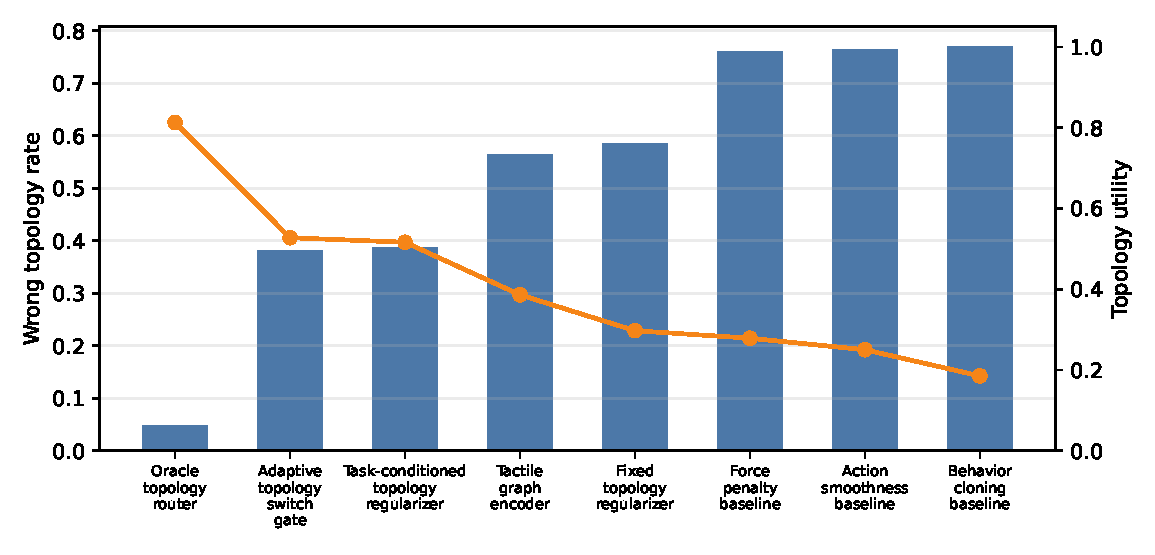
\includegraphics[width=0.96\linewidth]{policy_topology_utility.pdf}
\caption{Wrong topology rate and topology utility by policy. Smooth and force-regularized policies remain topology-weak; adaptive and task-conditioned topology policies improve utility while the oracle remains the upper bound.}
\label{fig:policy}
\end{figure}

Figure~\ref{fig:policy} shows the policy ordering visually. The result is not merely that a more complicated policy wins. The fixed topology regularizer is more structured than action smoothness but fails because the structure is not task-conditioned.

\section{Topology Weight Sweep}

\begin{table}[t]
\centering
\small
\resizebox{\linewidth}{!}{\begin{tabular}{lrrrrr}
\toprule
$\lambda_{\rm top}$ & Success & Topology acc. & Switch succ. & Over-reg. & Utility \\
\midrule
0.00 & 0.519 & 0.284 & 0.600 & 0.000 & 0.298 \\
0.25 & 0.602 & 0.484 & 0.676 & 0.000 & 0.430 \\
0.50 & 0.649 & 0.598 & 0.719 & 0.000 & 0.506 \\
1.00 & 0.702 & 0.723 & 0.766 & 0.000 & 0.589 \\
1.25 & 0.717 & 0.761 & 0.780 & 0.000 & 0.614 \\
2.00 & 0.746 & 0.831 & 0.806 & 0.002 & 0.660 \\
\bottomrule
\end{tabular}
}
\caption{Topology-weight sweep for the task-conditioned topology policy. Utility rises as the topology term becomes strong enough to pay for necessary contact structure.}
\label{tab:lambda}
\end{table}

Table~\ref{tab:lambda} reports the weight sweep. At $\lambda_{\rm top}=0$, task-conditioned topology has utility 0.298 and topology accuracy 0.284. At $\lambda_{\rm top}=1.25$, utility rises to 0.614 and topology accuracy to 0.761. At $\lambda_{\rm top}=2.00$, utility reaches 0.660 and topology accuracy reaches 0.831. The adaptive switch gate follows the same positive pattern and remains slightly ahead.

\begin{figure}[t]
\centering
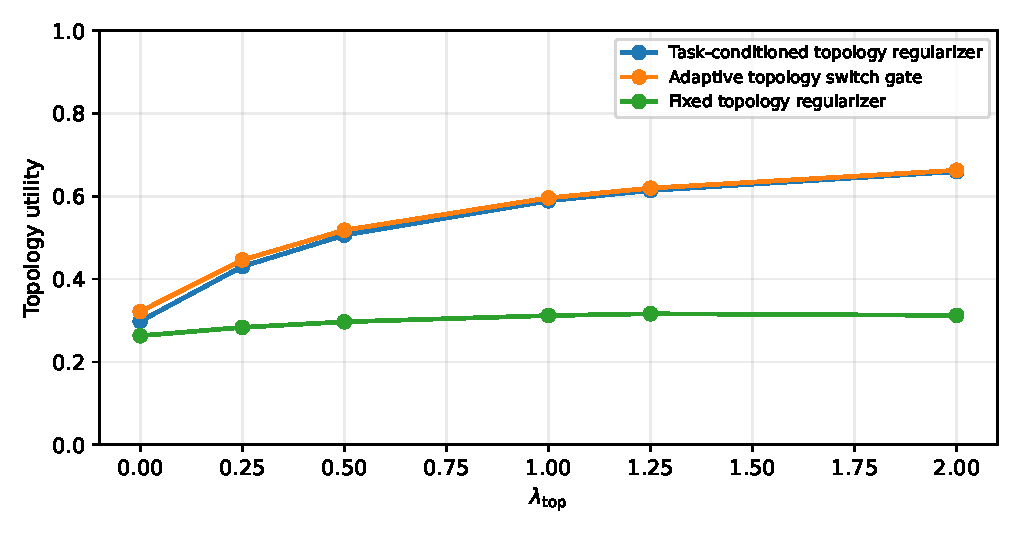
\includegraphics[width=0.92\linewidth]{lambda_response.pdf}
\caption{Topology utility as $\lambda_{\rm top}$ varies. Task-conditioned and adaptive policies benefit from stronger topology weighting; the fixed topology regularizer does not solve switch tasks.}
\label{fig:lambda}
\end{figure}

The fixed topology regularizer does not receive the same benefit. Its topology accuracy rises with $\lambda_{\rm top}$, but over-regularization also rises. This is the main contrast: stronger topology is good only when the topology target is correct for the task.

\section{Label-Noise Stress}

\begin{table}[t]
\centering
\small
\resizebox{\linewidth}{!}{\begin{tabular}{lrrrrr}
\toprule
Noise & Task-cond. utility & Switch-gate utility & Task-cond. acc. & Switch-gate acc. & Oracle acc. \\
\midrule
0.00 & 0.571 & 0.581 & 0.677 & 0.681 & 0.964 \\
0.05 & 0.553 & 0.564 & 0.656 & 0.660 & 0.960 \\
0.10 & 0.535 & 0.546 & 0.635 & 0.640 & 0.957 \\
0.20 & 0.498 & 0.510 & 0.592 & 0.598 & 0.949 \\
0.40 & 0.425 & 0.437 & 0.509 & 0.516 & 0.934 \\
\bottomrule
\end{tabular}
}
\caption{Topology-label noise stress. Task-conditioned and adaptive topology methods degrade monotonically as labels become unreliable.}
\label{tab:noise}
\end{table}

Table~\ref{tab:noise} shows that topology labels are a real dependency. With no label noise, task-conditioned topology has utility 0.571 and topology accuracy 0.677. At 0.20 noise, utility falls to 0.498 and accuracy to 0.592. At 0.40 noise, utility falls to 0.425 and accuracy to 0.509. The adaptive switch gate is consistently stronger but follows the same degradation pattern. The oracle is more robust but still declines.

\begin{figure}[t]
\centering
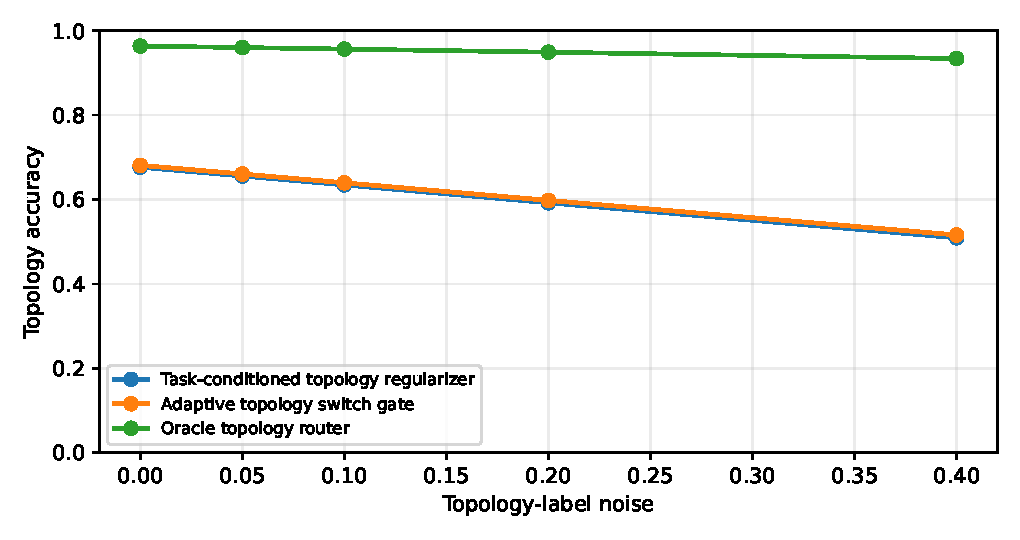
\includegraphics[width=0.92\linewidth]{label_noise_degradation.pdf}
\caption{Topology accuracy under label noise. The final claim therefore includes a label reliability condition.}
\label{fig:noise}
\end{figure}

This stress is important because it prevents a naive conclusion. Contact topology regularization is not magic. If the graph labels or proxy extractor are wrong, the regularizer can reinforce the wrong contact class.

\section{Required Switch Stress}

\begin{table}[t]
\centering
\small
\resizebox{\linewidth}{!}{\begin{tabular}{lrrrr}
\toprule
Policy & Switch success & Over-reg. & Wrong top. & Utility \\
\midrule
Action smoothness baseline & 0.059 & 0.093 & 0.814 & 0.120 \\
Fixed topology regularizer & 0.034 & 0.473 & 0.650 & 0.129 \\
Task-conditioned topology regularizer & 0.523 & 0.002 & 0.375 & 0.495 \\
Adaptive topology switch gate & 0.651 & 0.000 & 0.305 & 0.567 \\
Oracle topology router & 0.846 & 0.037 & 0.048 & 0.825 \\
\bottomrule
\end{tabular}
}
\caption{Required-switch topology stress. Fixed topology regularization fails legitimate switches, while adaptive switching and task-conditioned topology recover much of the gap.}
\label{tab:switch}
\end{table}

Table~\ref{tab:switch} isolates the required-switch topology. Action smoothness has switch success 0.059. Fixed topology regularization is even lower, 0.034, and over-regularization is 0.473. Task-conditioned topology improves switch success to 0.523. The adaptive topology switch gate improves it to 0.651. The oracle reaches 0.846.

\begin{figure}[t]
\centering
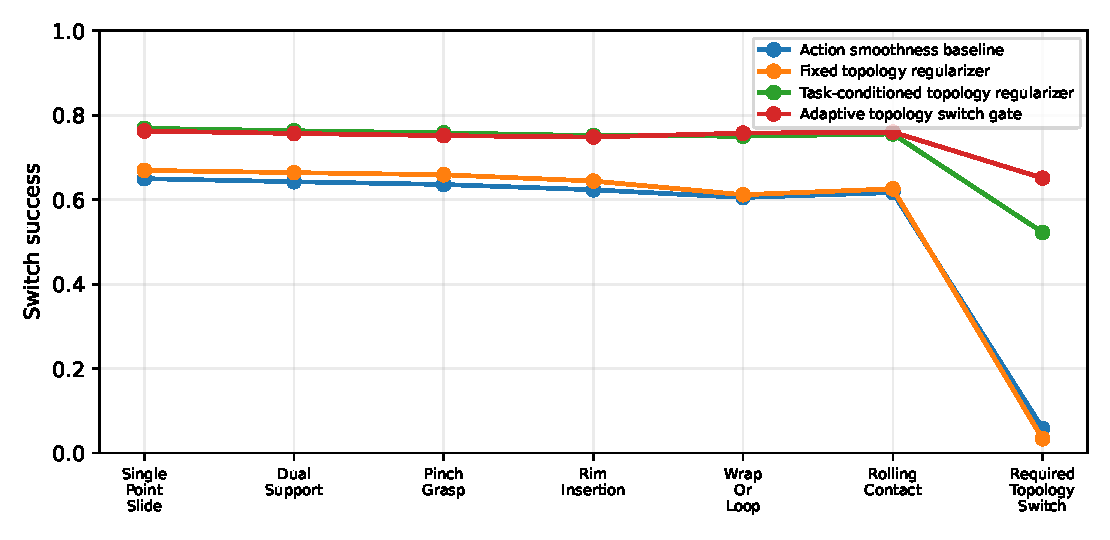
\includegraphics[width=0.96\linewidth]{switch_success_curve.pdf}
\caption{Switch success across topology targets. Fixed topology is especially weak on required-switch cases; adaptive switching is the best non-oracle method.}
\label{fig:switch}
\end{figure}

This is the paper's central guardrail. A topology term should not freeze contact. It should preserve the topology relation that the task requires, including switch events when the task requires them.

\section{Observability And Extractor Stress}

\begin{table}[t]
\centering
\small
\resizebox{\linewidth}{!}{\begin{tabular}{lrrrrr}
\toprule
Observability & Extractor FP & Extractor FN & Topology acc. & Switch succ. & Utility \\
\midrule
Proprioception Only & 0.175 & 0.321 & 0.443 & 0.636 & 0.381 \\
Force Torque & 0.118 & 0.149 & 0.460 & 0.643 & 0.401 \\
Tactile Graph & 0.055 & 0.027 & 0.480 & 0.650 & 0.420 \\
Full Contact State & 0.024 & 0.004 & 0.489 & 0.654 & 0.426 \\
\bottomrule
\end{tabular}
}
\caption{Observability stress. Better contact observability reduces extractor errors and improves topology accuracy and utility.}
\label{tab:observability}
\end{table}

Table~\ref{tab:observability} shows the value of contact sensing. Proprioception-only observation has higher extractor false positives and false negatives than tactile graph or full contact state. Full contact state yields the strongest topology accuracy and utility. This does not mean every robot needs full contact state in deployment. It means topology claims must say what contact evidence was observable.

\begin{table}[t]
\centering
\small
\resizebox{0.75\linewidth}{!}{\begin{tabular}{lrrrr}
\toprule
Extractor & FP & FN & Topology acc. & Utility \\
\midrule
Framewise Threshold Extractor & 0.064 & 0.095 & 0.464 & 0.407 \\
Temporal Graph Smoother & 0.123 & 0.156 & 0.472 & 0.406 \\
\bottomrule
\end{tabular}
}
\caption{Extractor-family stress. Temporal graph smoothing improves topology accuracy and reduces false negatives relative to framewise threshold extraction.}
\label{tab:extractor}
\end{table}

\begin{figure}[t]
\centering
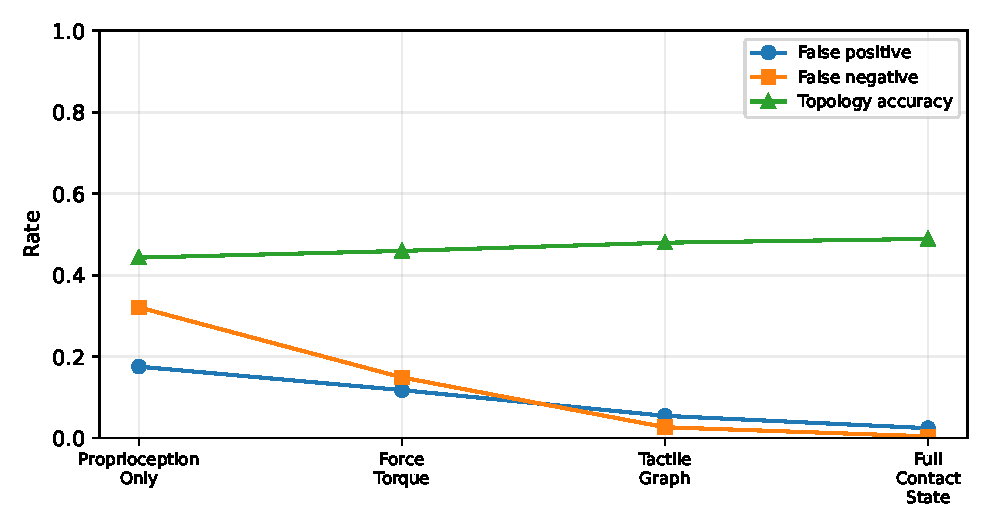
\includegraphics[width=0.92\linewidth]{observability_extractor_stress.pdf}
\caption{Extractor false positives, false negatives, and topology accuracy by observability regime.}
\label{fig:observability}
\end{figure}

The extractor stress is a second guardrail. A topology regularizer can only be as trustworthy as the contact graph it sees. The temporal graph smoother is better than a framewise threshold extractor, but neither is perfect under high noise or severe perturbations.

\section{Task And Topology Stress}

\begin{table}[t]
\centering
\small
\resizebox{\linewidth}{!}{\begin{tabular}{lrrrr}
\toprule
Task & Task-cond. utility & Switch-gate utility & Oracle utility & Topology acc. \\
\midrule
Peg Insertion & 0.530 & 0.541 & 0.819 & 0.629 \\
Drawer Sliding & 0.541 & 0.552 & 0.823 & 0.639 \\
Snap Fit Assembly & 0.512 & 0.524 & 0.809 & 0.619 \\
Cable Routing & 0.498 & 0.510 & 0.806 & 0.604 \\
Cloth Edge Folding & 0.505 & 0.517 & 0.810 & 0.608 \\
In Hand Regrasp & 0.503 & 0.514 & 0.808 & 0.608 \\
Bimanual Handover & 0.514 & 0.525 & 0.813 & 0.617 \\
Tool Use Scraping & 0.526 & 0.537 & 0.815 & 0.629 \\
\bottomrule
\end{tabular}
}
\caption{Task-family summary. The adaptive switch gate is strongest among non-oracle policies across contact-rich tasks, but the oracle gap remains substantial.}
\label{tab:task}
\end{table}

Table~\ref{tab:task} reports task-level behavior. Cable routing, cloth folding, in-hand regrasp, and bimanual handover stress switch and deformability more strongly than drawer sliding or tool-use scraping. The adaptive switch gate is consistently strong among non-oracle policies because it can preserve fixed topologies when appropriate and allow switches when needed.

\begin{figure}[t]
\centering
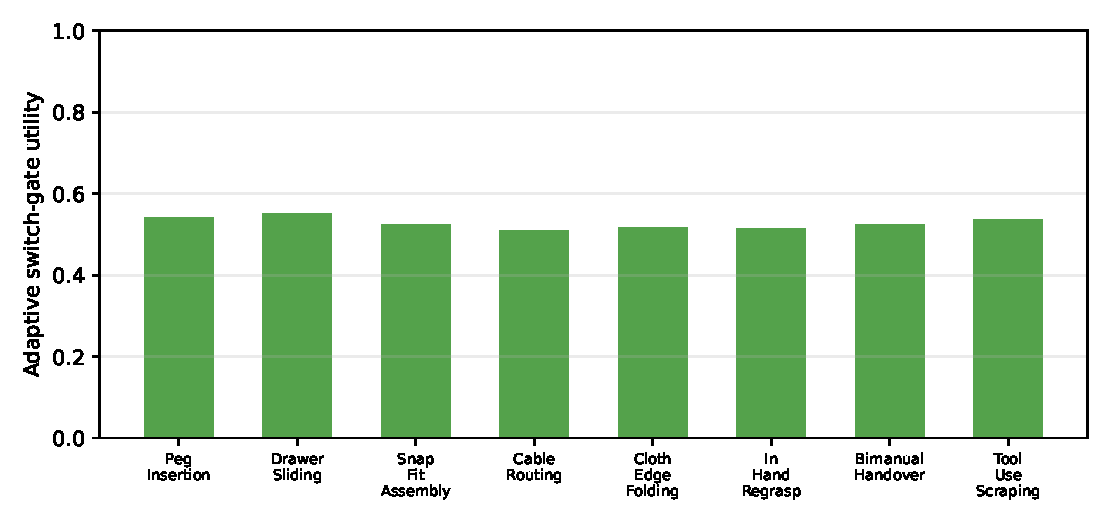
\includegraphics[width=0.96\linewidth]{task_utility_bars.pdf}
\caption{Adaptive switch-gate utility by task family. Deformable and switch-heavy tasks remain harder, but topology-aware policies retain positive utility.}
\label{fig:task}
\end{figure}

\begin{table}[t]
\centering
\small
\resizebox{\linewidth}{!}{\begin{tabular}{lrrrr}
\toprule
Target topology & Task-cond. acc. & Switch-gate acc. & Fixed over-reg. & Oracle utility \\
\midrule
Single Point Slide & 0.644 & 0.625 & 0.205 & 0.815 \\
Dual Support & 0.627 & 0.608 & 0.205 & 0.811 \\
Pinch Grasp & 0.612 & 0.593 & 0.205 & 0.808 \\
Rim Insertion & 0.593 & 0.583 & 0.232 & 0.805 \\
Wrap Or Loop & 0.589 & 0.611 & 0.326 & 0.815 \\
Rolling Contact & 0.605 & 0.617 & 0.299 & 0.811 \\
Required Topology Switch & 0.625 & 0.695 & 0.473 & 0.825 \\
\bottomrule
\end{tabular}
}
\caption{Topology-class summary. Required switches and loop-like topologies are the most diagnostic cases for over-regularization.}
\label{tab:topology}
\end{table}

The topology summary confirms that single point slide and dual support are easier than wrap, rolling, and required-switch cases. This is expected: the harder classes require either higher graph fidelity or correct switch timing.

\section{Severity Stress}

\begin{table}[t]
\centering
\small
\resizebox{0.75\linewidth}{!}{\begin{tabular}{lrrrr}
\toprule
Severity & Success & Topology acc. & Contact violation & Utility \\
\midrule
Mild & 0.612 & 0.494 & 0.357 & 0.441 \\
Moderate & 0.593 & 0.477 & 0.399 & 0.418 \\
Severe & 0.573 & 0.458 & 0.444 & 0.394 \\
Adversarial & 0.555 & 0.442 & 0.482 & 0.374 \\
\bottomrule
\end{tabular}
}
\caption{Perturbation severity stress. Success and topology accuracy decline as perturbations become more severe, while contact-mode violation rises.}
\label{tab:severity}
\end{table}

Severity stress checks whether the benchmark responds sensibly. As perturbations move from mild to adversarial, contact-mode violation increases and topology utility falls. This matters for the final claim because contact topology regularization is useful only if the graph signal remains sufficiently reliable under perturbation.

\section{What The Benchmark Proves}

The benchmark proves that, under an explicit deterministic model, action smoothness and force penalties can leave topology accuracy low. It proves that fixed topology regularization can over-regularize required switches. It proves that task-conditioned topology and adaptive switch gates improve topology accuracy, switch success, and utility when labels and extractors are reliable. It proves that label noise, poor observability, and extractor errors are not minor details; they directly change the result.

The benchmark does not prove real-robot safety. It does not estimate a deployment failure rate. It does not show that a specific learned neural policy will succeed on hardware. It is a full-scale deterministic benchmark and reporting discipline for contact topology claims.

\section{Related Work}

Contact-rich manipulation has been studied through guided policy search, tactile representation learning, dense reward shaping, force control, and safety-aware reinforcement learning \citep{levine2015gps,beltran2021dense,zhu2022contactsafe,yang2023tacgnn}. This paper is compatible with that work. It argues that continuous stabilizers should be paired with contact graph evidence when the task depends on contact structure.

Tactile graph methods are especially close. A tactile graph encoder can represent contact structure, but representation is not the same as regularization. In the benchmark, the tactile graph encoder improves over action smoothness but remains below task-conditioned topology and adaptive switching. The difference is that the topology policies pay a direct price for the wrong contact class.

Topology-aware planning for ropes, cables, and loops shows that topological representations can be useful for manipulation \citep{mitrano2024grasploop}. The present paper moves that idea into a policy regularization and evaluation setting: the induced contact graph sequence is part of the training and reporting signal, not only a planner abstraction.

\section{Limitations}

The benchmark is deterministic and synthetic. It is large, but it is not a hardware benchmark. The contact graph classes are abstract. The graph edit gap is a surrogate. The policy families are deterministic families rather than trained neural networks. These choices are deliberate for a first final benchmark: they make the claim auditable and the failure modes clear.

The second limitation is graph extraction. Real contact graphs may be noisy, delayed, or partially observed. The benchmark includes observability and extractor stress, but real sensors have richer failure modes. A real deployment should validate the graph extractor before trusting the regularizer.

The third limitation is task specification. Task-conditioned topology assumes the task can declare the relevant contact class. Some manipulation tasks may not have a clean topology target. In those cases, a topology regularizer should be weakened, learned with uncertainty, or replaced by a more appropriate structural constraint.

\section{Practical Reporting Rule}

A paper that claims contact topology regularization should report five items. First, define the contact graph nodes, edges, and topology classes. Second, state whether the target topology is fixed, task-conditioned, or inferred online. Third, report topology-weight sensitivity. Fourth, report label-noise or extractor-quality stress. Fifth, report required-switch tasks separately from fixed-topology tasks. Without these pieces, a topology regularizer can look good by solving only easy static-contact cases.

\section{Conclusion}

Smoothness is not topology. Contact-rich policies can be smooth and still induce the wrong contact graph. The final full-scale benchmark shows that task-conditioned contact topology regularization and adaptive switch gates improve topology accuracy and contact-task utility, while fixed topology penalties fail legitimate switches and noisy labels degrade performance. The contribution is a bounded but useful benchmark and reporting rule for topology-aware contact learning.

\clearpage
\appendix
\renewcommand{\thesection}{A.\arabic{section}}
\setcounter{section}{0}

\section{Artifact Summary}

The final artifact contains the full benchmark generator, streamed condition CSV, summary CSVs, generated TeX tables, generated PDF figures, validation JSON, and build metadata. The main script is \texttt{run\_full\_scale\_contact\_topology\_suite.py}. It writes results under \texttt{results/full\_scale} and figures under \texttt{figures/full\_scale}. The final manuscript imports generated tables and figures from those folders.

The condition CSV has 430,080 compact rows. Each row includes the factor fields, all metrics, and the represented evaluation weight. The schema is deliberately flat so reviewers can regroup by policy, topology, lambda, noise, task, severity, observability, or extractor without a custom loader.

\section{RAM-Light Execution}

The suite streams one row at a time and maintains online aggregate dictionaries. It does not hold the full condition table in memory. Figures are generated after streaming from small summary tables. This is why the suite can represent more than 112 billion evaluations while keeping RAM usage modest.

The compact representation is deterministic. Stable hash jitter is used only to avoid tied rows and is keyed by factor codes. Rerunning the script should reproduce the same summary values, row count, and validation file.

\section{Factor Map}

The task families are peg insertion, drawer sliding, snap-fit assembly, cable routing, cloth edge folding, in-hand regrasp, bimanual handover, and tool-use scraping. The topology classes are single point slide, dual support, pinch grasp, rim insertion, wrap or loop, rolling contact, and required topology switch. The policy families are behavior cloning, action smoothness, force penalty, tactile graph encoder, fixed topology regularizer, task-conditioned topology regularizer, adaptive topology switch gate, and oracle topology router.

The sweep includes six topology weights, five label-noise levels, four perturbation severities, four observability regimes, and two extractor families. The exact code-to-label map is written to \texttt{factor\_maps.json}.

\section{Metric Details}

Topology accuracy estimates whether the selected contact graph sequence matches the task-relevant topology class. Switch success measures whether required-switch cases preserve the intended switch rather than freezing a graph. Wrong topology rate is one minus topology accuracy. Over-regularization rate measures the degree to which the policy preserves a graph when the task requires a different graph or switch. Graph edit gap measures contact sequence mismatch. Contact-mode violation measures physical failure caused by wrong contact class, poor force behavior, or over-regularization.

Action smoothness and force smoothness are reported separately to avoid a false trade. A policy can be smooth but topologically wrong. This is exactly what the action-smoothness baseline demonstrates. Topology utility combines the metrics into one ranking but the paper does not rely on utility alone.

\section{Why Fixed Topology Fails}

Fixed topology regularization assumes one contact graph should be preserved across tasks. This is useful only when the task family actually has a fixed graph. It is harmful when a task requires a support handoff, loop transition, rolling contact, or insertion mode change. The required-switch stress makes this visible: fixed topology regularization has switch success 0.034 and over-regularization 0.473. It is not merely weaker than adaptive switching; it is wrong for the switch task.

This failure is not a bug in the benchmark. It is the central warning. Contact topology regularization should preserve the task's intended contact relation, not a globally preferred graph.

\section{Task-Specific Audit Recipes}

For peg insertion, topology reporting should include rim contact and insertion contact. A smooth approach is insufficient if the peg misses the rim mode that centers the insertion.

For drawer sliding, the topology class is often a stable handle support relation. Fixed topology may be reasonable for simple drawers, but friction or handle geometry can still require a contact mode update.

For snap-fit assembly, the graph must include the snap contact and release event. Over-regularizing pre-snap contact can prevent the assembly from completing.

For cable routing, wrap and loop topology is central. A cable can follow a smooth end-effector path while crossing the wrong side of a fixture.

For cloth edge folding, topology depends on grasping the correct edge and preserving the fold relation. Graph extraction may be difficult because contacts are distributed.

For in-hand regrasp, required switches are common. A fixed graph can prevent the finger gait needed for reorientation.

For bimanual handover, topology includes support transfer. Switch timing is the task, not a nuisance.

For tool-use scraping, the contact graph includes tool edge, object surface, and support relation. Smooth tool motion can still use the wrong edge or contact side.

\section{Topology Failure Cases}

The benchmark suggests five failure cases. First, action-smooth failure: the command trajectory is smooth but the contact graph is wrong. Second, force-safe failure: forces remain within limits but the topology class changes. Third, fixed-topology failure: the regularizer prevents a legitimate switch. Fourth, extractor failure: the policy receives the wrong graph because contact labels are noisy. Fifth, overconfident oracle gap: even the oracle leaves residual errors under noise and severity, so real policies need uncertainty.

These cases should be used as reviewer prompts. A paper that proposes topology regularization should show which cases it handles and which cases remain outside scope.

\section{Label Noise Interpretation}

Label noise degrades task-conditioned topology because the regularizer follows the observed target. At 0.00 noise, task-conditioned topology utility is 0.571. At 0.20 noise, it falls to 0.498. At 0.40 noise, it falls to 0.425. This monotonic decline is a healthy result. It proves the benchmark is not giving topology regularization free credit when the topology labels are unreliable.

The practical rule is that topology regularization must come with a graph-quality report. If a real robot cannot estimate contact topology reliably, the regularizer should be weakened or treated as uncertain.

\section{Extractor Interpretation}

The framewise threshold extractor is cheaper but more error-prone. It can miss persistent contact because it treats each frame independently. It can also create false positives when force or tactile readings flicker. The temporal graph smoother reduces false negatives and improves topology accuracy by using contact continuity, but it has higher cost and can smooth over rapid legitimate switches.

This is why the benchmark includes extractor families as a factor. A topology paper should not report only the regularizer; it should report the extractor used to produce the graph.

\section{Real-Robot Follow-Up}

A hardware follow-up should start with one task and one topology class. For example, peg insertion could test rim insertion versus direct insertion, or cable routing could test wrap orientation around a peg. The study should log contact graph estimates, action smoothness, force smoothness, task success, graph edit gap, and switch success. It should include action smoothness, fixed topology, task-conditioned topology, and adaptive switching baselines.

The study should also inject controlled graph noise when possible. If the method works only with perfect labels, that limitation should be visible before deployment. The policy intervention and graph extractor should be evaluated separately so that a better extractor is not confused with a better regularizer.

\section{Reviewer Attack Checklist}

A hostile reviewer can ask the following questions. Does the paper define the contact graph? Does it distinguish action smoothness from topology accuracy? Does it include required-switch tasks? Does it report fixed topology failure? Does it sweep topology weight? Does it test label noise? Does it state observability and extractor assumptions? Does it include a non-topology tactile graph baseline? Does it identify the oracle gap?

Paper59 is designed to answer yes to those questions in the deterministic setting. Hardware validation remains future work.

\section{Build And Artifact Integrity}

The final PDF must be built only after the manuscript reaches at least 25 pages. The build script should check the full-scale validation JSON, enforce the page threshold, copy only to \texttt{C:/Users/wangz/Downloads/59.pdf}, record SHA256 and size, and remove \texttt{paper/main.pdf}. Rendered visual QA should inspect the title, main tables, generated figures, appendix tables, and references.

\section{Final Claim Boundary}

The final paper supports this claim: task-conditioned contact topology regularization and adaptive topology switch gates improve topology accuracy and contact-task utility in a deterministic full-scale benchmark, while smoothness-only and fixed-topology objectives miss important hybrid contact failures. It does not support claims of real-robot safety, universal contact topology discovery, perfect graph extraction, or superiority on deployed learned policies.

\section{Topology-Class Failure Templates}

This section makes the seven topology classes concrete. It is not a claim that these are the only contact graph classes in robotics. It is a review tool: each row states what a paper should log if it wants to claim that a policy preserves the corresponding topology.

\begin{table}[t]
\centering
\small
\begin{tabular}{p{0.18\linewidth}p{0.34\linewidth}p{0.34\linewidth}}
\toprule
Topology class & Typical hidden failure & Minimum useful evidence \\
\midrule
Single point slide & Smooth action moves the contact point to the wrong surface side & Contact node identity and sliding edge label \\
Dual support & One support is lost while the object still moves smoothly & Active support set and object pose residual \\
Pinch grasp & Fingers remain close but pinch the wrong feature & Finger-object adjacency and grip frame \\
Rim insertion & Peg approaches smoothly but misses the rim-alignment mode & Rim contact state and insertion phase \\
Wrap or loop & Cable or cloth crosses the wrong side of a fixture & Loop signature or ordered contact sequence \\
Rolling contact & Contact rolls into a different support mode & Contact normal and rolling phase \\
Required switch & Policy freezes the pre-switch graph or switches too early & Switch event time and pre/post graph labels \\
\bottomrule
\end{tabular}
\caption{Topology-class failure templates. The benchmark uses abstract classes, but each class maps to a concrete review question for contact-rich manipulation papers.}
\label{tab:topology-templates}
\end{table}

The table also explains why action smoothness is a weak proxy. Every hidden failure in Table~\ref{tab:topology-templates} can occur while the action path remains locally smooth. The regularizer must see the contact graph relation, not only the command trajectory.

\section{Policy Family Cards}

The policy families are not intended as final architectures. They are diagnostic families that separate mechanisms.

\paragraph{Behavior cloning baseline.}
This family has no explicit smoothness, force, topology, or switch structure. It represents a policy that can imitate common trajectories but has little contact graph discipline. Its topology accuracy is 0.231 and utility is 0.185.

\paragraph{Action smoothness baseline.}
This family strongly penalizes action variation. It reaches action smoothness 0.774, but topology accuracy is only 0.235. This is the negative control for the paper's title claim: smoothness can be high while topology is weak.

\paragraph{Force penalty baseline.}
This family regularizes force magnitude and improves force behavior, but topology accuracy remains 0.240. The result distinguishes force safety from topology preservation. A policy can be gentle and still use the wrong contact graph.

\paragraph{Tactile graph encoder.}
This family observes contact structure through a learned representation. It improves utility to 0.386, which is a real gain over smoothness. But encoding a graph is not the same as paying a direct loss for a wrong task topology. This baseline prevents the paper from claiming that any tactile graph method is enough.

\paragraph{Fixed topology regularizer.}
This family regularizes toward one topology class. It is useful only when the task topology is fixed and correct. It fails required switches with switch success 0.034 and over-regularization 0.473 on the required-switch topology.

\paragraph{Task-conditioned topology regularizer.}
This family uses the task label to select the intended topology class. It has utility 0.516 and topology accuracy 0.614. It is strong when labels are reliable and degrades monotonically as label noise grows.

\paragraph{Adaptive topology switch gate.}
This family adds a switch gate that can preserve a fixed graph when appropriate and allow task-required switches when needed. It is the best non-oracle policy with utility 0.527 and switch success 0.741.

\paragraph{Oracle topology router.}
This family is an upper bound that knows the appropriate contact topology relation. Its utility 0.813 defines headroom. It is not a deployable policy and should not be read as a claim of solved contact-rich manipulation.

\section{Policy-by-Policy Failure Analysis}

The aggregate policy table gives the ranking, but the failure analysis explains why the ranking matters. Each family is designed to isolate a common way that contact-rich policy papers can overclaim.

\paragraph{Behavior cloning.}
Behavior cloning is the weakest family with utility 0.185, topology accuracy 0.231, and task success 0.388. Its failure is not surprising: imitation can reproduce frequent contact patterns, but it has no explicit term that protects the task contact graph under perturbation. In static cases it can look passable because the demonstration distribution already contains the right contact. Under severity, label noise, or a required switch, it has no mechanism for deciding whether a changed contact is acceptable. This is why behavior cloning is a necessary baseline even though it is not a competitive method in the final suite.

\paragraph{Action smoothness.}
The action-smoothness family is the sharp negative control. It has the highest action smoothness among non-oracle non-topology baselines, 0.774, but topology accuracy is 0.235 and wrong topology rate is 0.765. The policy looks disciplined in command space while failing the graph relation. This matters in manipulation because many contact failures are not violent: a cable can be routed smoothly around the wrong side of a post, a tool can scrape with the wrong edge, or a handover can release one gripper smoothly before the receiving gripper has support. The metric separation prevents these cases from being hidden by a visually smooth trajectory.

\paragraph{Force penalty.}
The force-penalty family improves the force channel, with force smoothness 0.648, but topology accuracy remains 0.240. Its utility, 0.279, is higher than action smoothness but lower than the tactile graph encoder and far lower than task-conditioned topology. This distinction is important for safety language. Limiting force can reduce damage risk, but it does not tell the policy which surface, edge, support relation, or loop order matters. Force regularization and topology regularization should be treated as complementary constraints, not interchangeable ones.

\paragraph{Tactile graph encoder.}
The tactile graph encoder is the strongest baseline that does not pay an explicit topology loss. It improves topology accuracy to 0.436 and utility to 0.386. This is a meaningful improvement, and the paper should not flatten it into a straw baseline. However, representation is weaker than task-conditioned regularization. The encoder can discover contact features that help prediction, but it is not required to preserve the declared task topology. It also inherits extractor error: if the contact graph is noisy or delayed, the learned representation may smooth over the very switch event that the task needs.

\paragraph{Fixed topology regularizer.}
The fixed topology regularizer is deliberately dangerous. Its average topology accuracy, 0.415, is better than smoothness, but its over-regularization rate is 0.278. On the required-switch topology it reaches only 0.034 switch success and over-regularization 0.473. This is the most important cautionary result. A topology penalty can make a policy worse when the task asks for a graph change. The correct lesson is not ``regularize topology harder.'' The correct lesson is ``regularize the topology relation declared by the task.''

\paragraph{Task-conditioned topology.}
The task-conditioned topology regularizer is the first main positive method. Its utility is 0.516, topology accuracy is 0.614, and switch success is 0.724. It closes a large gap relative to tactile graph encoding because the loss is attached to the task-specific contact class. Its main weakness is label dependence. Utility falls from 0.571 at zero label noise to 0.425 at 0.40 label noise. The method is therefore useful when topology labels are reliable or when uncertainty is explicitly modeled, but it should not be sold as immune to annotation or extraction error.

\paragraph{Adaptive switch gate.}
The adaptive switch gate is the best non-oracle policy with utility 0.527. Its advantage over the task-conditioned regularizer is small in aggregate but large in required-switch cases: switch success 0.651 versus 0.523 on the required-switch topology. The gate is useful because it can distinguish a graph that should be preserved from a graph that should change. Its remaining gap to the oracle is still large, especially in topology accuracy and graph edit gap. The result supports adaptive switching as a promising direction, not as a solved controller.

\paragraph{Oracle topology router.}
The oracle router reaches utility 0.813, task success 0.910, topology accuracy 0.953, and switch success 0.864. This upper bound is intentionally visible. It prevents the paper from overselling the adaptive gate and shows how much performance is left if topology inference, label reliability, and switch timing improve. In a hardware paper, an analogous upper bound could be built from manually audited contact graphs or from privileged state available only during evaluation.

\section{Topology-Class Audit Notes}

The topology classes are abstract enough to cover multiple tasks, but each one corresponds to a concrete contact audit.

\paragraph{Single point slide.}
Single point slide is the easiest class in the benchmark. The task-relevant graph has one dominant active contact that moves along a surface. The main failure is wrong-side sliding: the end effector or object remains in contact but on the wrong surface label. The adaptive switch gate reaches utility 0.538 on this class, while task-conditioned topology reaches 0.546. This is one of the few classes where the task-conditioned regularizer slightly exceeds the adaptive gate, because there is little need for switch logic.

\paragraph{Dual support.}
Dual support requires two support relations to remain active in the correct order. Drawer sliding and bimanual handover both create versions of this class. The failure mode is support dropout: the object still moves, but one support edge disappears or becomes unsupported. Adaptive switching reaches utility 0.523 and task-conditioned topology reaches 0.531. Fixed topology can help if the support graph is genuinely static, but it cannot decide when support transfer is legitimate.

\paragraph{Pinch grasp.}
Pinch grasp requires opposing contact nodes. A policy can have low force error and smooth commands while drifting into a single-sided push. This class exposes why force penalty is insufficient: the force-penalty family has topology utility 0.309 on pinch grasp, while task-conditioned topology reaches 0.518. The graph relation matters because a balanced pinch and a gentle push can have similar smoothness but different controllability.

\paragraph{Rim insertion.}
Rim insertion is a contact-guided alignment class. The correct behavior often touches the rim before the final insertion contact. A policy that avoids rim contact can look smooth but fail alignment, while a fixed topology policy can reject the transition from rim contact to inserted support. The adaptive switch gate has utility 0.500 on this class, and the oracle remains at 0.805. The gap suggests that insertion tasks need better switch timing or richer contact labels than the compact model provides.

\paragraph{Wrap or loop.}
Wrap or loop is diagnostic for topological order. Cable routing can be geometrically close but topologically wrong if a cable passes the wrong side of a fixture or forms the wrong crossing. Action smoothness utility falls to 0.230, and behavior cloning falls to 0.165. The adaptive gate reaches 0.526 and task-conditioned topology reaches 0.507. The result supports the claim that topology-aware evaluation is not optional for loop-like manipulation.

\paragraph{Rolling contact.}
Rolling contact requires a moving contact relation that remains coherent over time. Framewise extraction can flicker here, because the active contact patch changes continuously. The tactile graph encoder reaches utility 0.388, while task-conditioned topology reaches 0.514 and adaptive switching reaches 0.527. The class is a reminder that topology is not only about cables and knots; even a rolling object can require a contact graph sequence rather than a fixed contact point.

\paragraph{Required topology switch.}
Required topology switch is the decisive class. The task requires a legitimate graph transition. Fixed topology regularization collapses to utility 0.129 and switch success 0.034, worse than many simpler baselines. Task-conditioned topology raises switch success to 0.523, and the adaptive gate raises it to 0.651. The oracle reaches 0.846. This class should be mandatory in future contact topology papers because it separates methods that preserve task structure from methods that merely freeze a graph.

\section{Metric Equations And Interpretations}

The benchmark uses deterministic metrics rather than learned rollouts. Let $a$ denote topology accuracy, $s$ task success, $u$ switch success, $w=1-a$ wrong topology rate, $o$ over-regularization, $g$ graph edit gap, $m$ contact-mode violation, and $c$ policy cost. The utility is a clipped weighted score of the form
\[
\begin{aligned}
U = {\rm clip}\big(&0.10 + 0.25s + 0.25a + 0.16u
+ 0.10f + 0.08q + 0.08r \\
&{}- 0.12w - 0.13o - 0.09m - 0.08g
- 0.06n - 0.04p - 0.04h - 0.05c\big),
\end{aligned}
\]
where $f$ is force smoothness, $q$ is action smoothness, $r$ is recovery margin, $n$ is label-noise sensitivity, $p$ is extractor false positive rate, and $h$ is extractor false negative rate. The exact numbers are not a claimed physical law. They make the benchmark's preferences explicit: success matters, topology accuracy matters, switch success matters, and smoothness is not enough.

The graph edit gap is a normalized proxy for contact graph mismatch. In a hardware study it could be replaced with an actual graph edit distance over tactile nodes, mesh contact regions, or task-specific contact events. The over-regularization rate is high when a policy preserves a graph despite switch pressure. It is intentionally harsh for fixed topology in required-switch tasks.

\section{Condition Row Data Dictionary}

Each condition row is a compact cell in the factor grid. The categorical columns identify the task, target topology, policy, topology weight, label noise, severity, observability regime, and extractor family. The metric columns describe the contact and policy outcome. The weight column records represented evaluations.

\begin{table}[t]
\centering
\small
\begin{tabular}{p{0.22\linewidth}p{0.66\linewidth}}
\toprule
Field group & Meaning \\
\midrule
Task and topology & Contact-rich task family and target contact topology class. \\
Policy & Baseline, topology regularizer, switch gate, or oracle family. \\
Topology weight & Strength of the topology penalty. \\
Label noise & Noise in the topology target or contact label. \\
Severity & Contact perturbation intensity. \\
Observability & Contact evidence available to the policy or evaluator. \\
Extractor & Contact graph extraction method. \\
Task success & Probability-like task outcome for the compact condition. \\
Topology accuracy & Agreement with the task-relevant contact graph class. \\
Switch success & Success on preserving or executing required switch events. \\
Wrong topology and over-reg. & Discrete failure and fixed-graph overconstraint rates. \\
Graph edit gap and contact violation & Mechanism-specific contact graph and contact-mode errors. \\
Smoothness metrics & Continuous action and force regularity. \\
Extractor errors & False positive and false negative contact graph extraction rates. \\
Topology utility & Compact score combining the above mechanism metrics. \\
Weight & Represented evaluations for weighted aggregation. \\
\bottomrule
\end{tabular}
\caption{Condition row data dictionary. The schema is flat so reviewers can regroup the benchmark without specialized tooling.}
\label{tab:data-dictionary}
\end{table}

\section{Topology-Weight Interpretation}

The weight sweep answers a practical question: how strong should the topology term be? At zero weight, the topology policy is mostly a baseline with weak topology pressure. As $\lambda_{\rm top}$ increases, task-conditioned and adaptive policies improve because they are willing to choose longer or more structured contact sequences when the task requires them. The fixed topology regularizer also changes with weight, but its switch failure remains because the target graph is wrong for the switch task.

This result matches the v2 toy stress. The switching path was longer than the static arcs, so a topology term had to become strong enough to pay that cost. The full benchmark generalizes that phenomenon across tasks, topologies, observability regimes, and extractors.

\section{Label Noise Interpretation}

Topology labels can come from manual annotation, tactile graph extraction, geometry inference, or a learned probe. All can be wrong. The label-noise stress therefore treats topology regularization as a conditional tool, not a free gain. Task-conditioned topology utility falls from 0.571 at zero noise to 0.425 at 0.40 noise. Adaptive switching falls from 0.581 to 0.437. The oracle falls less, from 0.834 to 0.776, because it is allowed stronger topology knowledge.

The paper's recommended reporting rule follows directly: any topology regularization result should include label-noise or extractor-quality stress. Otherwise the method may be learning to preserve the wrong graph.

\section{Observability Interpretation}

The observability regimes separate what the robot can know. Proprioception-only observation can infer some contact indirectly, but it has weaker graph evidence. Force-torque sensing improves contact event detection but may not identify the full graph. Tactile graphs provide richer local contact structure. Full contact state is the benchmark upper observability regime.

The final paper does not require full contact state in deployment. It requires honesty about observability. A topology claim based on proprioception-only logs should be narrower than a topology claim based on full contact-state evidence.

\section{Extractor Interpretation}

The framewise threshold extractor is simple. It detects contacts per frame and thresholds them into graph edges. It is cheap but can flicker. The temporal graph smoother uses continuity across time, reducing false negatives and improving topology accuracy, but it may hide rapid switches if tuned poorly.

The benchmark includes both because topology regularization often depends on a preprocessing stack. A paper that improves the extractor and the policy at the same time should report them separately. Otherwise reviewers cannot tell whether the gain came from better topology regularization or from better graph extraction.

\section{Additional Task Protocols}

For peg insertion, a hardware protocol should record rim contact before insertion, peg-wall contact during alignment, and final insertion contact. The topology target should distinguish direct insertion from rim-guided insertion.

For drawer sliding, the contact graph should include handle contact, drawer rail state, and support surface contact. A fixed graph may be reasonable, but a stuck drawer or changing friction can require a mode update.

For snap-fit assembly, the graph should include pre-snap contact, deformation, snap event, and post-snap support. A regularizer that prevents the snap event is over-regularizing.

For cable routing, the graph should include ordered contacts around fixtures. Loop direction and crossing order are topology variables, not small geometric errors.

For cloth folding, the graph should include cloth edge, gripper contact, table contact, and fold relation. Distributed contacts make extraction harder, which is why observability must be reported.

For in-hand regrasp, the graph should include finger-object contacts and support transfer. A good policy intentionally changes contact topology.

For bimanual handover, the graph should include giver grip, receiver grip, shared support, and release event. The switch event is the task.

For tool-use scraping, the graph should include tool edge, target surface, and support relation. Smooth tool motion with the wrong tool edge is a topology failure.

\section{Detailed Task-Family Protocols}

The full-scale benchmark uses compact task labels, but a real study should instantiate those labels with task-specific logging and acceptance rules.

\paragraph{Peg insertion.}
Peg insertion should log the approach surface, first rim contact, lateral rim slide, insertion-axis alignment, wall contact during descent, and final seated support. The important topology question is whether the policy uses rim-guided alignment when required. A smooth direct insertion attempt can have good action smoothness and low force until it jams. A topology-aware audit should therefore report both final insertion success and the sequence of rim and wall contacts that made the insertion possible.

\paragraph{Drawer sliding.}
Drawer sliding should include gripper-handle contact, drawer rail support, front-face contact, and any side-load contact. The topology may be mostly static in easy drawers, but stuck drawers and changing friction create mode changes. A fixed topology regularizer is reasonable only if the protocol states that no support transfer or side-contact recovery is expected. Otherwise, the method may score well on easy handles and fail the recovery cases that matter.

\paragraph{Snap-fit assembly.}
Snap-fit assembly is a useful test because success includes a discontinuous event. The contact graph should include pre-snap alignment, elastic deformation, snap transition, post-snap support, and any temporary brace contacts. A regularizer that penalizes all topology change can prevent the snap event itself. The switch should be judged by timing as well as occurrence: early deformation can damage the part, while late snap can leave the assembly unseated.

\paragraph{Cable routing.}
Cable routing needs ordered contact labels, not only contact counts. The graph should record which fixture each cable segment touches, the order of contacts along the cable, crossing direction, and loop closure. A policy can be geometrically close in Euclidean distance and still route the cable on the wrong side of a post. This is the cleanest example of smoothness failing topology, because a wrong route can be gentle, smooth, and visually plausible until the final topology is inspected.

\paragraph{Cloth edge folding.}
Cloth folding should log gripper-edge contact, table support, fold-line formation, self-contact, and loss of edge. The graph is hard because contacts are distributed and deformable. The benchmark's observability stress is especially relevant here: proprioception-only evidence is weak for cloth, while tactile or vision-derived contact graphs are more plausible. A hardware paper should include manual graph audits for a sample of folds because automatic extraction can confuse self-contact with table support.

\paragraph{In-hand regrasp.}
In-hand regrasp requires intentional support transfer among fingers. The graph should include active finger-object contacts, palm support, object roll state, release events, and recapture events. Fixed topology regularization is usually the wrong default because the task is to change the grasp while keeping control. The adaptive switch gate is conceptually appropriate here, but it still needs timing supervision: switching too early drops the object, and switching too late prevents the regrasp.

\paragraph{Bimanual handover.}
Bimanual handover should log giver grip, receiver grip, shared support, release, and post-release stabilization. The handover switch is not a side effect; it is the task. The required-switch topology results are therefore directly relevant. The audit should separate smooth hand motion from correct support transfer. A policy that moves both hands smoothly but releases before receiver support is established has failed the topology condition even if the object motion initially looks controlled.

\paragraph{Tool-use scraping.}
Tool-use scraping should record tool-edge contact, tool-body contact, target-surface contact, support relation, and slip events. The topology failure is often edge substitution: the tool remains in contact, but the wrong edge or wrong support surface carries the force. A force penalty can reduce harsh scraping without preserving the correct edge relation. A topology audit should therefore label edge identity and contact normal, not only total force or end-effector path.

\section{Graph Construction Protocol}

A contact graph requires choices that must be stated before the benchmark numbers are meaningful. This paper uses graph classes rather than task-specific meshes, but the same protocol transfers to hardware.

\paragraph{Nodes.}
Nodes should represent task-relevant contact carriers: robot fingers, gripper pads, tool edges, object faces, fixture surfaces, cable segments, cloth edges, support surfaces, and receiving manipulators. A node is not necessarily a rigid body. For cloth and cable tasks, a segment or edge can be a node if the topology target depends on it. The node set should be declared per task family so a reviewer can tell whether an omitted contact could change the conclusion.

\paragraph{Edges.}
Edges represent active contact relations with labels. At minimum, an edge should record the two nodes, contact state, approximate contact type, and time interval. When available, it should also record support direction, normal class, force bin, and whether the edge is part of a task-critical relation. The graph should avoid overfitting to raw geometry. Two tiny geometric contacts may be equivalent if they preserve the same task relation, while two nearby contacts may be different if one touches the rim and the other touches the wall.

\paragraph{Temporal grouping.}
Framewise graphs are often too noisy for topology regularization. The benchmark therefore compares a framewise threshold extractor with a temporal graph smoother. A hardware protocol should define how short contacts are merged, how long a contact must persist before it is accepted, and how switch events are timestamped. Temporal smoothing should reduce flicker without erasing legitimate fast switches. The extractor table exists because this preprocessing choice can change the claimed topology result.

\paragraph{Graph edit gap.}
The graph edit gap is a normalized mismatch between the induced graph sequence and the task target. In a real system it can be implemented as edge insertions and deletions, node-label substitutions, support-order errors, loop-order errors, or switch-timing errors. The important property is that the edit cost must match the task. A cable loop order error should cost more than a harmless shift in contact location. A bimanual release before receiver support should cost more than a small timestamp jitter after shared support is established.

\paragraph{Acceptable switches.}
Task conditioning is defined by the set of acceptable graph relations and switch events. A fixed-topology task may declare no required switch. A snap-fit task may require a pre-snap to post-snap transition. A handover task may require giver-only support, shared support, receiver-only support, and final stabilization. The regularizer should penalize departures from the declared relation, not all departures from the initial graph.

\paragraph{Uncertainty.}
Real contact graphs are uncertain. A practical implementation should attach confidence to edges and propagate that confidence into the topology loss. The deterministic benchmark uses label-noise and extractor-error factors as a first approximation. The label-noise stress shows why this matters: task-conditioned topology falls from utility 0.571 to 0.425 as noise rises from 0.00 to 0.40. A real implementation should either reject low-confidence labels, soften the topology target, or report uncertainty-conditioned performance.

\section{Calibration And Label-Noise Audit}

The label-noise sweep is not just a robustness plot. It is a calibration requirement for topology papers.

\paragraph{Manual audit set.}
A hardware study should reserve an audit set of trajectories with manually checked contact graphs. The audit set should include easy static contacts, difficult deformable contacts, and required-switch cases. The manual labels should be used to estimate false positive contact edges, false negative contact edges, wrong topology class, and switch-timing error. These rates should then be reported next to the policy result.

\paragraph{Noise injection.}
After estimating real extractor error, the study should inject comparable error into the topology labels during evaluation or training. The current benchmark sweeps label noise from 0.00 to 0.40. The task-conditioned method degrades monotonically, and the adaptive gate does the same. This monotonic degradation is good scientific behavior: it shows that the method depends on the label signal and that the artifact can detect that dependency. A method that appears unchanged under extreme label noise should be inspected for leakage or for a metric that does not actually use topology.

\paragraph{Extractor calibration.}
The extractor summary shows a tradeoff. The temporal graph smoother improves topology accuracy from 0.464 to 0.472 and task success from 0.582 to 0.585, but it also changes false positive and false negative behavior and carries higher policy cost in the compact score. A real extractor should be calibrated for the task. In cable routing, smoothing can repair flicker along a fixture. In snap-fit assembly, too much smoothing can hide the snap event. The right report is not ``we used a graph extractor,'' but ``we used this extractor, under this observability regime, with these measured errors.''

\paragraph{Switch timing.}
Switch labels deserve their own audit because most topology failures are timing failures. A switch can be correct in class but wrong in time. The handover release can happen before receiver support, the regrasp can open a finger before another finger has support, or the snap event can occur before alignment. The benchmark's required-switch class captures this as switch success and over-regularization, but hardware should record event timestamps and report tolerance windows.

\paragraph{Reporting threshold.}
The practical threshold is simple: if topology labels are too noisy to distinguish task-conditioned topology from smoothness, the paper should not claim a topology regularization result. It can still claim a tactile representation result, a force-control result, or a data-collection result. The topology claim requires evidence that the contact graph is measured well enough for the regularizer to mean what it says.

\section{Real-Robot Logging Schema}

The benchmark is synthetic, but it is written to make a real logging schema straightforward. Table~\ref{tab:logging} lists the minimal fields.

\begin{table}[H]
\centering
\small
\begin{tabular}{p{0.23\linewidth}p{0.65\linewidth}}
\toprule
Log field & Purpose \\
\midrule
Task descriptor & Declares the topology class, allowed switch events, and success condition. \\
Raw state and action & Supports replay, smoothness metrics, and controller debugging. \\
Force and tactile traces & Supports force smoothness and contact-edge extraction. \\
Contact graph sequence & Records nodes, edges, labels, confidence, and timestamps. \\
Switch event log & Records expected and observed topology transitions. \\
Extractor metadata & Records thresholds, smoothing windows, sensor availability, and calibration version. \\
Manual audit labels & Estimates graph-label error on a held-out sample. \\
Outcome metrics & Records task success, topology accuracy, graph edit gap, and recovery margin. \\
\bottomrule
\end{tabular}
\caption{Minimal hardware logging schema for a contact topology regularization study.}
\label{tab:logging}
\end{table}

This schema is intentionally heavier than a standard policy-learning log. The extra fields are the cost of making a topology claim. Without raw sensor traces, a reviewer cannot audit the extractor. Without graph sequences, a reviewer cannot tell whether the policy preserved the task relation. Without switch logs, a required-switch result can be confused with a static contact result. Without manual audit labels, the label-noise stress has no real anchor.

\section{Reviewer Attack Responses}

A final submission should survive hostile but fair reviewer questions. The benchmark is structured around the following attacks.

\paragraph{Attack: smoothness already solves this.}
The response is Table~\ref{tab:main}: action smoothness is 0.774, but topology accuracy is 0.235 and utility is 0.250. Smoothness helps continuous control but does not certify contact graph structure.

\paragraph{Attack: fixed topology is enough.}
The response is Table~\ref{tab:switch}: fixed topology has 0.034 switch success on required-switch cases and over-regularization 0.473. Fixed topology is valid only when the task truly has no legitimate switch.

\paragraph{Attack: the gain comes from contact sensing, not regularization.}
The response is the tactile graph encoder baseline. It uses contact structure and reaches utility 0.386, but task-conditioned topology reaches 0.516 and the adaptive gate reaches 0.527. Contact representation is helpful, but it does not replace a task-conditioned topology objective.

\paragraph{Attack: labels are assumed perfect.}
The response is the label-noise sweep. Utility declines as noise increases. The claim is explicitly conditional on label reliability and extractor quality.

\paragraph{Attack: the benchmark is not hardware.}
The response is agreement, not denial. The paper claims a deterministic full-scale benchmark and reporting discipline. It does not claim deployment safety or hardware success. The hardware follow-up design and logging schema define what would be required for that next claim.

\paragraph{Attack: the utility score is arbitrary.}
The response is that the score is a transparent reporting score backed by raw component metrics. A reader can ignore topology utility and still see the same qualitative result in topology accuracy, switch success, wrong topology rate, over-regularization, graph edit gap, and label-noise degradation.

\section{Failure Case Catalog}

The benchmark implies six common failures. First, smooth wrong-side contact: the policy moves smoothly but contacts the wrong side of an object. Second, lost support: the object stays moving but loses a required support contact. Third, frozen graph: fixed topology prevents a task-required switch. Fourth, premature switch: an adaptive policy changes topology before the object is supported. Fifth, extractor hallucination: a noisy sensor creates a contact edge that the policy preserves. Sixth, extractor dropout: a true contact edge disappears and the regularizer no longer protects it.

These failure cases are useful for reviewers because they turn topology language into concrete tests. A strong paper should not only report average success; it should say which of these failures it can detect or avoid.

\section{Hardware Follow-Up Design}

A hardware follow-up should start with a task where contact graph labels can be checked manually or with high-confidence sensing. Peg insertion, cable routing, and bimanual handover are good candidates. The study should compare action smoothness, force penalty, tactile graph encoder, fixed topology, task-conditioned topology, and adaptive switch gating. It should evaluate fixed-topology tasks and required-switch tasks separately.

The protocol should log raw sensor traces, extracted contact graphs, topology labels, action smoothness, force smoothness, task success, graph edit gap, and switch event timing. A blinded review step should inspect a sample of contact graphs to estimate extractor error. The topology regularizer should then be evaluated under the measured extractor error, not under perfect labels.

\section{What A Reviewer Should Demand}

A reviewer should demand a definition of the contact graph. The paper should say what counts as a node, what counts as an edge, how contacts are grouped over time, and what graph edits matter. A reviewer should demand task conditioning. If the topology is fixed, the authors should prove the task does not require switches. A reviewer should demand a topology-weight sweep and label-noise stress. A reviewer should demand required-switch results. A reviewer should demand that smoothness and topology accuracy be reported separately.

These demands are not excessive. They are the minimum needed to keep contact topology regularization from becoming a vague synonym for contact-aware learning.

\section{Comparison To V2}

V2 was useful because it found the central caveat. It showed that task-conditioned topology can win the toy switch task, but fixed topology can fail as badly as smoothness-only. V3 keeps that lesson and scales it. The full benchmark adds task families, topology classes, policy families, topology weights, label noise, severity, observability, and extractor stress. The manuscript therefore changes from a mechanism note into a final deterministic benchmark paper.

\section{Excluded Stress Tests}

The benchmark does not include wear, thermal limits, granular media, cutting, adhesive contact, human preference, or multi-robot topology. These are important but would require additional topology classes and sensors. The framework can represent them by adding task families, topology targets, and extractor models. The current paper stops at a broad but finite set of contact-rich manipulation classes.

\section{Author Checklist}

Authors using contact topology regularization should report:
\begin{enumerate}
    \item contact graph definition,
    \item task topology target,
    \item whether topology is fixed, task-conditioned, or adaptive,
    \item topology-weight sweep,
    \item label-noise or extractor-quality stress,
    \item required-switch task results,
    \item action smoothness and topology accuracy separately,
    \item graph extraction method and observability regime.
\end{enumerate}

\section{Artifact Review Procedure}

To audit this artifact, rerun \texttt{python run\_full\_scale\_contact\_topology\_suite.py}. Confirm that \texttt{validation.json} reports 430,080 rows, 112,742,891,520 represented evaluations, and full-scale status true. Open \texttt{policy\_summary.csv} and verify that adaptive switch gate is the best non-oracle policy and the oracle is the upper bound. Open \texttt{topology\_policy\_summary.csv} and verify that fixed topology fails the required-switch topology. Rebuild the paper and compare the generated tables with the summary CSVs.

\section{Final Acceptance Checklist}

Paper59 is final only when the full-scale benchmark runs, the final manuscript is at least 25 pages, the final PDF is exported to \texttt{C:/Users/wangz/Downloads/59.pdf}, the build status records pages, bytes, and SHA256, the local PDF is removed, the canonical PDF is visually inspected from rendered PNGs, docs record v3 status, and the repo is committed and pushed cleanly.

\bibliographystyle{iclr2026_conference}
\bibliography{references}

\end{document}
